% This template was initially provided by Dulip Withanage.
% Modifications for the database systems research group
% were made by Conny Junghans,  Jannik Strötgen and Michael Gertz

\documentclass[
     12pt,         % font size
     a4paper,      % paper format
     BCOR10mm,     % binding correction
     DIV14,        % stripe size for margin calculation
     ]{article}

%%%%%%%%%%%%%%%%%%%%%%%%%%%%%%%%%%%%%%%%%%%%%%%%%%%%%%%%%%%%

% PACKAGES:

% Use German :
\usepackage[english]{babel}
% Input and font encoding
\usepackage[latin1]{inputenc}
\usepackage[T1]{fontenc}
% Index-generation
\usepackage{makeidx}
% Einbinden von URLs:
\usepackage{url}
% Special \LaTex symbols (e.g. \BibTeX):
%\usepackage{doc}
% Include Graphic-files:
\usepackage{graphicx}
% Include doc++ generated tex-files:
%\usepackage{docxx}

% Fuer anderthalbzeiligen Textsatz
\usepackage{setspace}

% hyperrefs in the documents
\PassOptionsToPackage{hyphens}{url}\usepackage[bookmarks=true,colorlinks,pdfpagelabels,pdfstartview = FitH,bookmarksopen = true,bookmarksnumbered = true,linkcolor = black,plainpages = false,hypertexnames = false,citecolor = black,urlcolor=black]{hyperref}
%\usepackage{hyperref}

%%%%%%%%%%%%%%%%%%%%%%%%%%%%%%%%%%%%%%%%%%%%%%%%%%%%%%%%%%%%

% OTHER SETTINGS:

% Choose language
\newcommand{\setlang}[1]{\selectlanguage{#1}\nonfrenchspacing}


\begin{document}

% TITLE:
\pagenumbering{roman} 
\begin{titlepage}


\vspace*{1cm}
\begin{center}
\vspace*{3cm}
\textbf{ 
\Large Heidelberg University\\
\smallskip
\Large Institute of Computer Science\\
\smallskip
\Large Database Systems Research Group\\
\smallskip
}

\vspace{3cm}

\textbf{\large Project Proposal for the lecture Text Analytics}

\vspace{0.5\baselineskip}
{\huge
\textbf{Working Title}
}
\end{center}

\vfill 

{\large
\begin{tabular}[l]{ll}
Team Member: & Name, Matriculation Number, Course of Study\\
  & email address\\
Team Member: & Name, Matriculation Number, Course of Study\\
  & email address\\
Team Member: & Name, Matriculation Number, Course of Study\\
  & email address\\

% If the line goes too far to the right, you can alter this slightly, e.g.
Team Member: & Very long Name, Matriculation Number\\
  & Course of Study, email address\\
  
\end{tabular}
}

\end{titlepage}

\pagenumbering{arabic} 

\section{Introduction}
Motivate your project and state the \textit{real-world problem} you want to solve.

\section{Section}

Use sections to organize your contents. Read the project proposal guidelines available on Moodle to get more information on the contents your proposal should cover. Do not forget to cite online sources~\cite{WFR2017}, books~\cite{goldberg2017neural} or articles you are referencing! It may also be useful to integrate charts or figures in your proposal as seen in Figure~\ref{fig:example}.

\begin{figure}[h]
  \centering
  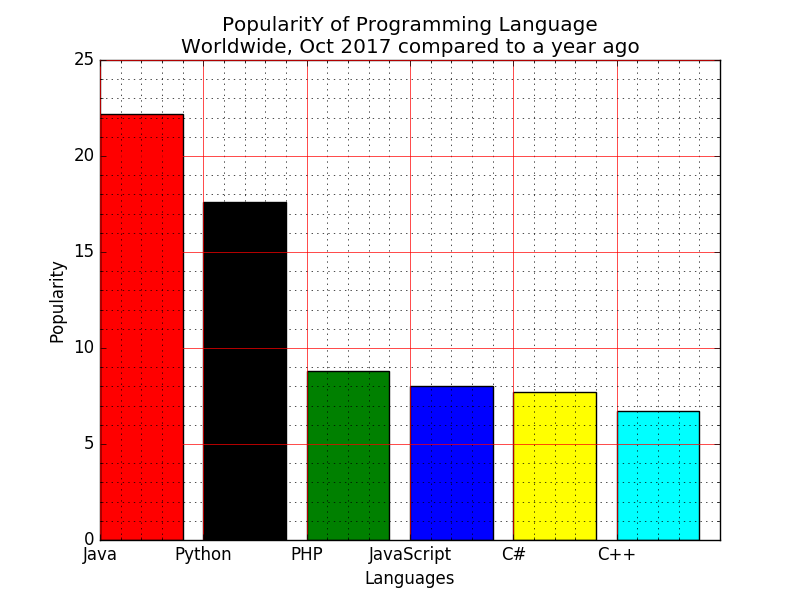
\includegraphics[scale=0.3]{figures/example_barchart}
  \caption[]{An example chart showing the change of popularity of various programming languages\footnotemark[1].}
  \label{fig:example}
\end{figure}

\footnotetext[1]{\url{https://www.w3resource.com/w3r_images/matplotlib-barchart-exercise-4.png}}

In the Latex source provided together with this PDF, you also find hints on how to work on one Latex project collaboratively.


%%%%%%%%%%%%%%%%%%%%%%%%%%%%%%%%%%%%%%%%%%%%%%%%%%%%%%%%%%%%

% The following is especially useful if you work together on one proposal or report, and want to alter its content independently from each other (e.g., to keep your commit history clean).

% Alternative: put content in separate files
% Check the difference between including these files using \input{filename} and \include{filename} and see which one you like better
%\chapter{Einleitung}\label{intro}
%\subsection{Introduction}

\subcomment{Written by Daniela Fichiu}
If you type a query like "how do I open the terminal on mac?" into Google, you already know what you want to find: a set of steps that will open a terminal on the screen.

Most would say doing homework is, on the best days, an unpleasant affair. But everyone would agree that writing an assignment for that one course you've always skipped is a chore. You most certainly do not understand the airy slides. Your only option is to search for materials on your own - extensive research is needed to find the materials that can fill all your knowledge gaps.

A student who wants to know more about text analytics might search for "text analytics" on Google Scholar. The query yields back 1.650.000 results, the top three being "Text Analytics with Python," "Text analytics in social media," and "Semantic interaction for visual text analytics." A subsequent query like "text analytics topics" yields back results with the following titles: "Analyzing educational comments for topics and sentiments: A text analytics approach" or "A text analytics approach for online retailing service improvement: Evidence from Twitter."

We know how time-consuming it is to spend hours on search engines or websites like Research Gate or Google Scholar looking for research papers, hoping for the best, but never quite finding the perfect materials.

Our project emerged from the need to find an easy way of exhaustively searching for scholarly literature while bringing to light the relations between the subfields of the research field of interest and other areas. Our goal is to provide a deeper understanding of the material to be searched for and easing up the process of finding information.

We propose a solution that clusters scientific texts into relevant subgroups. The subgroups can then be more easily presented to and explored by people looking for specific topics and terms.

We focus on a subset of around two thousand papers from the field of machine learning. We cluster the research papers, extract a ground truth using the papers' keywords, and compare the clustering results against the ground truth. We also prove that an unbalanced data set can have a significant impact on the clustering results. 

Even with the conclusions written down, we do not see our work as finished. The proposed pipeline could be usable on a broader range of fields. We also intend to balance our data set by adding research papers from other areas.

We also believe that our solution, supported by good group visualization tools and a user-friendly search interface, can be successfully integrated into a metasearch site.
%
%\chapter{Voraussetzungen}\label{bg}
%\input{background}

%%%%%%%%%%%%%%%%%%%%%%%%%%%%%%%%%%%%%%%%%%%%%%%%%%%%%%%%%%%%

% References (Literaturverzeichnis):
% see
% https://de.wikibooks.org/wiki/LaTeX-W%C3%B6rterbuch:_bibliographystyle
% for the different formats and styles

\bibliographystyle{plain}
% b) The File:
\bibliography{references}

\end{document}
